\title{MathRecap}
\author{fDero}

\newenvironment{sistema}%
{\left\lbrace\begin{array}{@{}l@{}}}%
{\end{array}\right.}

\begin{titlepage}
    \begin{center}
        \begin{tabular}{c}
            {https://www.github.com/fDero/MathRecap}         \\[70pt]
            {\Huge \bf Abstract Mathematical Studies}        \\[10pt]
            \hline                                           \\[20pt]
            {\bf \Large Francesco De Rosa | github: fDero}   \\[30pt]
            
            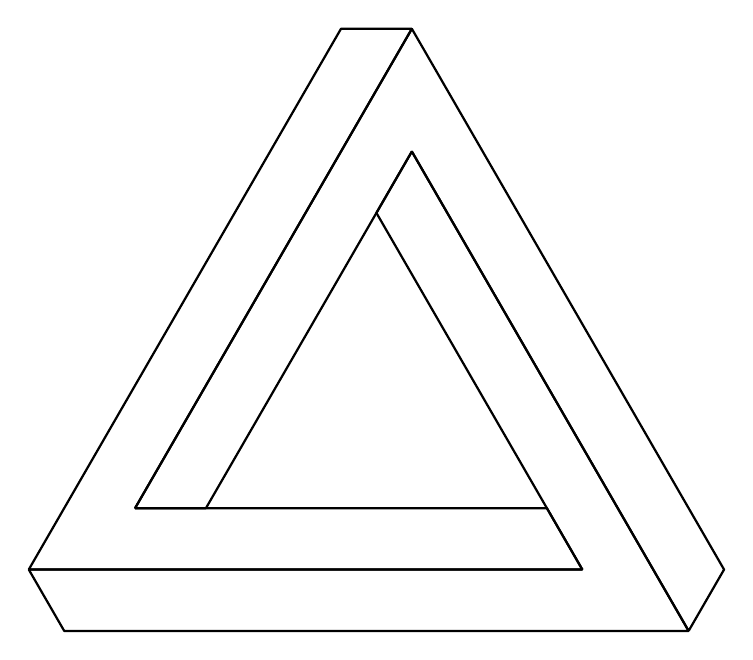
\begin{tikzpicture}[scale=1, line join=bevel]
	
                \pgfmathsetmacro{\a}{2.5}
                \pgfmathsetmacro{\b}{0.9}
            
                \tikzset{
                  apply style/.code     = {\tikzset{#1}},
                  triangle_edges/.style = {thick,draw=black}
                }
            
                \foreach \theta/\facestyle in {
                    0/{triangle_edges},
                  120/{triangle_edges},
                  240/{triangle_edges}
                }{
                    \begin{scope}[rotate=\theta]
                        \draw[apply style/.expand once=\facestyle]
                        ({-sqrt(3)/2*\a},{-0.5*\a})                   --
                        ++(-\b,0)                                     --
                        ({0.5*\b},{\a+3*sqrt(3)/2*\b})                --
                        ({sqrt(3)/2*\a+2.5*\b},{-.5*\a-sqrt(3)/2*\b}) --
                        ++({-.5*\b},-{sqrt(3)/2*\b})                  --
                        ({0.5*\b},{\a+sqrt(3)/2*\b})                  --
                        cycle;
                    \end{scope}
                }	
            \end{tikzpicture}      
        \end{tabular}
    \end{center}
\end{titlepage}